\section{Levi-Civita 联络}\label{sec:levi-civita-connection}

在 Riemann 流形上, 有一种特殊的联络, 称为 \textbf{Levi-Civita 联络}, 它具有特殊的几何性质.

\begin{RiemannDefinition}\label{def:metric-compatible-connection}
Riemann 流形 $(M,\langle\cdot,\cdot\rangle)$ 上的联络 $\nabla$ 称为\textbf{与度量相容}, 若下式对所有 $X,Y,Z\in\mathfrak{X}(M)$ 成立:
\[
  X\cdot\langle Y,Z\rangle
  =\langle\nabla_XY,Z\rangle+\langle Y,\nabla_XZ\rangle.
\]
\end{RiemannDefinition}

若 $\nabla$ 与度量相容, 则两个沿曲线平行的向量场 $V_1$ 和 $V_2$ 的内积沿该曲线为常数:
\[
  \frac{\mathrm{d}}{\mathrm{d}t}\langle V_1(t),V_2(t)\rangle
  =\bigl\langle\nabla_{\dot c(t)}V_1(t),V_2(t)\bigr\rangle
   +\bigl\langle V_1(t),\nabla_{\dot c(t)}V_2(t)\bigr\rangle=0.
\]
特别地, 平行移动保持向量的长度和向量间的夹角. 因此, 若 $c:I\to M$ 是一条测地线, 则 $\lVert\dot c(t)\rVert=k$ 为常数. 若 $a\in I$, 则测地线从 $a$ 到 $t$ 的长度 $s$ 为
\[
  s=\int_a^t\lVert\dot c(v)\rVert\,\mathrm{d}v
   =\int_a^t k\,\mathrm{d}v=k(t-a).
\]
换言之, $t$ 是弧长 $s$ 的仿射函数 (因而称为\textbf{仿射参数}). 特别地, 这说明像相同的两条测地线的参数互为仿射函数.

\begin{RiemannTheorem}[Levi–Civita]\label{thm:levi-civita-connection}
若 $(M,\langle\cdot,\cdot\rangle)$ 是 Riemann 流形, 则 $M$ 上存在唯一的对称且与 $\langle\cdot,\cdot\rangle$ 相容的联络 $\nabla$. 在局部坐标 $(x^1,\ldots,x^n)$ 下, 此联络的 Christoffel 符号为
\begin{equation}\label{eq:levi-civita-christoffel-symbols}
  \Gamma^i_{jk}=\frac12\sum_{l=1}^n g^{il}
  \left(\frac{\partial g_{kl}}{\partial x^j}
       +\frac{\partial g_{jl}}{\partial x^k}
       -\frac{\partial g_{jk}}{\partial x^l}\right)
\end{equation}
其中 $(g^{ij})=(g_{ij})^{-1}$.
\end{RiemannTheorem}

\begin{RiemannProof}
设 $X,Y,Z\in\mathfrak{X}(M)$. 若 Levi-Civita 联络存在, 则必有
\begin{align*}
  X\cdot\langle Y,Z\rangle &= \langle\nabla_XY,Z\rangle+\langle Y,\nabla_XZ\rangle;\\
  Y\cdot\langle X,Z\rangle &= \langle\nabla_YX,Z\rangle+\langle X,\nabla_YZ\rangle;\\
  -Z\cdot\langle X,Y\rangle &= -\langle\nabla_ZX,Y\rangle-\langle X,\nabla_ZY\rangle,
\end{align*}
因为 $\nabla$ 与度量相容. 此外, 由于 $\nabla$ 是对称的, 还必有
\begin{align*}
  -\langle[X,Z],Y\rangle &= -\langle\nabla_XZ,Y\rangle+\langle\nabla_ZX,Y\rangle;\\
  -\langle[Y,Z],X\rangle &= -\langle\nabla_YZ,X\rangle+\langle\nabla_ZY,X\rangle;\\
  \langle[X,Y],Z\rangle &= \langle\nabla_XY,Z\rangle-\langle\nabla_YX,Z\rangle.
\end{align*}
将这六个等式相加, 得到 \textbf{Koszul 公式}
\begin{align*}
  2\langle\nabla_XY,Z\rangle
    &= X\cdot\langle Y,Z\rangle+Y\cdot\langle X,Z\rangle-Z\cdot\langle X,Y\rangle\\
    &\quad-\langle[X,Z],Y\rangle-\langle[Y,Z],X\rangle+\langle[X,Y],Z\rangle.
\end{align*}
由于 $\langle\cdot,\cdot\rangle$ 非退化且 $Z$ 任意, 此公式确定了 $\nabla_XY$. 因此, Levi-Civita 联络若存在, 必是唯一的.

为证明存在性, 我们用 Koszul 公式\textbf{定义} $\nabla_XY$. 不难证明这确实定义了一个联络 [参见 \RiemannExercisePart{ex:koszul-defines-connection}]. 此外, 利用此公式可得
\[
  2\langle\nabla_XY-\nabla_YX,Z\rangle
  =2\langle\nabla_XY,Z\rangle-2\langle\nabla_YX,Z\rangle=2\langle[X,Y],Z\rangle
\]
对任意 $X,Y,Z\in\mathfrak{X}(M)$ 成立, 故 $\nabla$ 是对称的. 最后, 再用 Koszul 公式可得
\[
  2\langle\nabla_XY,Z\rangle+2\langle Y,\nabla_XZ\rangle=2X\cdot\langle Y,Z\rangle
\]
所以由此公式定义的联络与度量相容.

选取局部坐标 $(x^1,\ldots,x^n)$, 有
\[
  \left[\frac{\partial}{\partial x^i},\frac{\partial}{\partial x^j}\right]=0
  \quad\text{且}\quad
  \left\langle\frac{\partial}{\partial x^i},\frac{\partial}{\partial x^j}\right\rangle=g_{ij}.
\]
因此, Koszul 公式给出
\begin{gather*}
  2\left\langle\nabla_{\frac{\partial}{\partial x^j}}\frac{\partial}{\partial x^k},
    \frac{\partial}{\partial x^l}\right\rangle
    =\frac{\partial}{\partial x^j}\cdot g_{kl}
     +\frac{\partial}{\partial x^k}\cdot g_{jl}
     -\frac{\partial}{\partial x^l}\cdot g_{jk}\\
  \Leftrightarrow\
  \left\langle\sum_{i=1}^n\Gamma^i_{jk}\frac{\partial}{\partial x^i},
    \frac{\partial}{\partial x^l}\right\rangle
    =\frac12\left(\frac{\partial g_{kl}}{\partial x^j}
                 +\frac{\partial g_{jl}}{\partial x^k}
                 -\frac{\partial g_{jk}}{\partial x^l}\right)\\
  \Leftrightarrow\
  \sum_{i=1}^n g_{il}\Gamma^i_{jk}
    =\frac12\left(\frac{\partial g_{kl}}{\partial x^j}
                 +\frac{\partial g_{jl}}{\partial x^k}
                 -\frac{\partial g_{jk}}{\partial x^l}\right).
\end{gather*}
容易解出此线性方程组, 得到 \eqref{eq:levi-civita-christoffel-symbols}.
\end{RiemannProof}

\RiemannExerciseHeading
\begin{enumerate}[label=(\arabic*),ref=\arabic*,leftmargin=*]
\item\label{ex:koszul-defines-connection}
证明 Koszul 公式定义了一个联络.

\item\label{ex:euclidean-connection-with-torsion}
在赋有通常 Euclidean 度量 $\langle\cdot,\cdot\rangle$ 的 $\mathbb{R}^3$ 中, 引入联络 $\nabla$, 它在 Cartesian 坐标 $(x^1,x^2,x^3)$ 下由下式定义:
\[
  \Gamma^i_{jk}=\omega\varepsilon_{ijk},
\]
其中 $\omega:\mathbb{R}^3\to\mathbb{R}$ 是光滑函数, 且
\[
  \varepsilon_{ijk}=\begin{cases}
    +1 & \text{若 $(i,j,k)$ 是 $(1,2,3)$ 的偶置换},\\
    -1 & \text{若 $(i,j,k)$ 是 $(1,2,3)$ 的奇置换},\\
    0  & \text{其他情形}.
  \end{cases}
\]
证明:
\begin{enumerate}[label=(\alph*),leftmargin=*]
\item $\nabla$ 与 $\langle\cdot,\cdot\rangle$ 相容;
\item $\nabla$ 的测地线是直线;
\item 在所有满足 $\omega\ne 0$ 的点, $\nabla$ 的挠率均非零 (因此, 除非 $\omega\equiv 0$, 否则 $\nabla$ 不是 Levi-Civita 联络);
\item 平行移动方程为
\[
  \dot V^i+\sum_{j,k=1}^3\omega\varepsilon_{ijk}\dot x^j V^k=0
  \Leftrightarrow \dot V+\omega(\dot x\times V)=0
\]
(其中 $\times$ 是 $\mathbb{R}^3$ 中的叉积); 因此, 沿直线平行的向量以角速度 $-\omega\dot x$ 绕该直线旋转.
\end{enumerate}

\item\label{ex:isometry-preserves-levi-civita}
设 $(M,g)$ 与 $(N,\widetilde g)$ 是等距的 Riemann 流形, 其 Levi-Civita 联络分别为 $\nabla$ 和 $\widetilde\nabla$, 并设 $f:M\to N$ 是一个等距映射. 证明:
\begin{enumerate}[label=(\alph*),leftmargin=*]
\item 对任意 $X,Y\in\mathfrak{X}(M)$, 有 $f_*\nabla_XY=\widetilde\nabla_{f_*X}f_*Y$;
\item 若 $c:I\to M$ 是测地线, 则 $f\circ c:I\to N$ 也是测地线.
\end{enumerate}

\item\label{ex:spherical-geodesics-and-transport}
考虑 $S^2\subset\mathbb{R}^3$ 上通常的局部坐标 $(\theta,\varphi)$, 它由如下参数化 $\phi:(0,\pi)\times(0,2\pi)\to\mathbb{R}^3$ 定义:
\[
  \phi(\theta,\varphi)=(\sin\theta\cos\varphi,\sin\theta\sin\varphi,\cos\theta).
\]
\begin{enumerate}[label=(\alph*),leftmargin=*]
\item 用这些坐标确定 $\mathbb{R}^3$ 的 Euclidean 度量在 $S^2$ 上诱导的 Riemann 度量的表达式.
\item 计算这些坐标下 Levi-Civita 联络的 Christoffel 符号.
\item 证明赤道是某条测地线的像.
\item 证明 $\mathbb{R}^3$ 中绕任一过原点的轴的旋转都诱导 $S^2$ 的等距映射.
\item 证明 $S^2$ 的测地线的像为大圆.
\item 找出一个内角和为 $\frac{3\pi}{2}$ 的\textbf{测地三角形} (即三边均为测地线的像的三角形).
\item 令 $c:\mathbb{R}\to S^2$ 由 $c(t)=(\sin\theta_0\cos t,\sin\theta_0\sin t,\cos\theta_0)$ 给出, 其中 $\theta_0\in(0,\frac{\pi}{2})$ (因而 $c$ 不是测地线). 设 $V$ 是沿 $c$ 平行的向量场, 满足 $V(0)=\frac{\partial}{\partial\theta}$ ($\frac{\partial}{\partial\theta}$ 由连续性在 $(\sin\theta_0,0,\cos\theta_0)$ 处有良好定义). 计算 $V$ 回到起点时转过的角度.
{\small (\textbf{Remark:} 你所算出的角度, 恰好是在纬度 $\frac{\pi}{2}-\theta_0$ 处, \textbf{Foucault 摆}的振动平面在一天内转过的角度, 因为在自转的地球上, 该平面趋于相对恒星保持不动.)}
\item 利用这一结果证明: $S^2$ 中不存在与带 Euclidean 度量的 $\mathbb{R}^2$ 中某个开集 $W$ 等距的开集 $U$.
\item 在带 Euclidean 度量的 $\mathbb{R}^2$ 中, 给定测地线 $c:\mathbb{R}\to\mathbb{R}^2$ 和一点 $p\notin c(\mathbb{R})$, 存在唯一的测地线 $\widetilde c:\mathbb{R}\to\mathbb{R}^2$ (相差重新参数化), 使得 $p\in\widetilde c(\mathbb{R})$ 且 $c(\mathbb{R})\cap\widetilde c(\mathbb{R})=\varnothing$ (\textbf{平行公设}). 这在 $S^2$ 上也成立吗?
\end{enumerate}

\item\label{ex:hyperbolic-plane}
回顾一下, 将
\[
  H=\{(x,y)\in\mathbb{R}^2\mid y>0\}
\]
中的每一点与由 $h(t)=yt+x$ 给出的可逆仿射映射 $h:\mathbb{R}\to\mathbb{R}$ 等同, 就在 $H$ 上诱导了 Lie 群结构 [参见 Chapter~\RiemannSourceRef{chap:differentiable-manifolds} 的 Exercise~\RiemannSourceRef{ex:affine-maps-lie-group}].
\begin{enumerate}[label=(\alph*),leftmargin=*]
\item 证明: $\mathfrak h=T_{(0,1)}H$ 中的 Euclidean 内积 $\mathrm{d}x\otimes\mathrm{d}x+\mathrm{d}y\otimes\mathrm{d}y$ 所诱导的左不变度量为
\[
  g=\frac{1}{y^2}(\mathrm{d}x\otimes\mathrm{d}x+\mathrm{d}y\otimes\mathrm{d}y)
\]
[参见 Exercise~\RiemannSourceRef{ex:left-invariant-metric}]. {\small (\textbf{Remark:} 赋有此度量的 $H$ 称为\textbf{双曲平面}.)}
\item 计算坐标 $(x,y)$ 下 Levi-Civita 联络的 Christoffel 符号.
\item 证明在这些坐标下由
\begin{align*}
  \alpha(t)&=(0,e^t)\\
  \beta(t)&=\left(\tanh t,\frac{1}{\cosh t}\right)
\end{align*}
给出的曲线 $\alpha,\beta:\mathbb{R}\to H$ 是测地线. 集合 $\alpha(\mathbb{R})$ 和 $\beta(\mathbb{R})$ 是什么?
\item 确定所有测地线的像.
\item 证明: 给定 $p,q\in H$ 两点, 存在唯一的经过它们的测地线 (相差重新参数化).
\item 给出连通 Riemann 流形的例子, 其中有两点, (i) 有无穷多条测地线 (按重新参数化等同) 经过这两点; (ii) 没有测地线经过这两点.
\item 证明: $H$ 中不存在与带 Euclidean 度量的 $\mathbb{R}^2$ 中某个开集 $V$ 等距的开集 $U$. {\small (\textbf{Hint:} 证明任意一点 $p\in H$ 的任意邻域中, 总有一个内角和小于 $2\pi$ 的测地四边形.)}
\item 平行公设在双曲平面上成立吗?
\end{enumerate}

\item\label{ex:induced-connection-and-projection}
设 $(M,\langle\cdot,\cdot\rangle)$ 是 Levi-Civita 联络为 $\widetilde\nabla$ 的 Riemann 流形, 并设 $(N,\langle\langle\cdot,\cdot\rangle\rangle)$ 是带有诱导度量且 Levi-Civita 联络为 $\nabla$ 的子流形.
\begin{enumerate}[label=(\alph*),leftmargin=*]
\item 证明对任意 $X,Y\in\mathfrak{X}(N)$, 都有
\[
  \nabla_XY=\bigl(\widetilde\nabla_{\widetilde X}\widetilde Y\bigr)^{\top},
\]
其中 $\widetilde X,\widetilde Y$ 分别是 $X,Y$ 到 $\mathfrak{X}(M)$ 的任意延拓, 而 $\mathord{}^{\top}:TM|_N\to TN$ 是正交投影.
\item 利用这一结果, 分别举出 $\mathbb{R}^3$ 中下列曲面上是测地线的曲线以及不是测地线的曲线:
\begin{enumerate}[label=(\roman*),leftmargin=*]
\item 球面 $S^2$;
\item 旋转环面;
\item 锥面;
\item 一般的旋转曲面.
\end{enumerate}
\item 证明: 若 $\mathbb{R}^3$ 中的两个曲面沿一条曲线相切, 则向量沿该曲线在两个曲面上的平行移动相同.
\item 利用这一结果, 计算将向量 $V$ 沿球面上一个圆作平行移动时转过的角度 $\Delta\theta$.
{\small (\textbf{Hint:} 考虑沿该圆与球面相切的锥面 (参见 Fig.~\ref{fig:sphere-circle-parallel-transport}); 注意, 从该锥面去掉一条经过锥顶的射线之后得到的曲面, 与 Euclidean 平面中的一个开集等距.)}
\end{enumerate}

\item\label{ex:metric-is-parallel}
设 $(M,g)$ 是 Levi-Civita 联络为 $\nabla$ 的 Riemann 流形. 证明 $g$ 沿任意曲线\textbf{平行}, 即证明对任意 $X\in\mathfrak{X}(M)$ 都有
\[
  \nabla_Xg=0
\]
[参见 Exercise~\RiemannSourceRef{ex:covariant-derivative-of-tensors}].

\item\label{ex:killing-vector-field}
设 $(M,g)$ 是 Levi-Civita 联络为 $\nabla$ 的 Riemann 流形, $\psi_t:M\to M$ 是一个单参数等距变换群. 由
\[
  X_p:=\left.\frac{\mathrm{d}}{\mathrm{d}t}\right|_{t=0}\psi_t(p)
\]
定义的向量场 $X\in\mathfrak{X}(M)$ 称为与 $\psi_t$ 对应的 \textbf{Killing 向量场}. 证明:
\begin{enumerate}[label=(\alph*),leftmargin=*]
\item $L_Xg=0$ [参见 Exercise~\RiemannSourceRef{ex:lie-derivative-of-tensors}];
\item 对任意向量场 $Y,Z\in\mathfrak{X}(M)$, $X$ 满足 $\langle\nabla_YX,Z\rangle+\langle\nabla_ZX,Y\rangle=0$;
\begin{figure}[htbp]
  \centering
  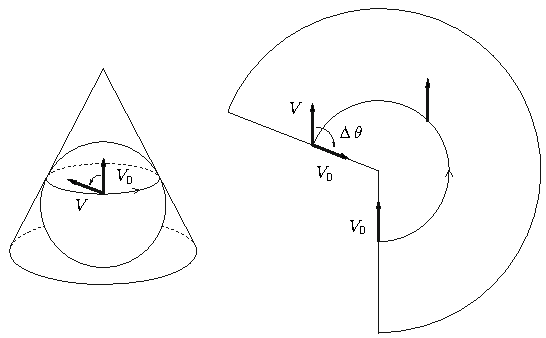
\includegraphics[width=.54\textwidth]{figures/parallel-transport-sphere.pdf}
  \caption{沿球面上一个圆的平行移动}\label{fig:sphere-circle-parallel-transport}
\end{figure}
\item 若 $c:I\to M$ 是测地线, 则 $\langle\dot c(t),X_{c(t)}\rangle$ 是常数.
\end{enumerate}

\item\label{ex:riemannian-divergence-trace}
回顾一下, 若 $M$ 是带有体积元 $\omega\in\Omega^n(M)$ 的定向微分流形, 则 $X$ 的\textbf{散度}是满足
\[
  L_X\omega=(\operatorname{div}(X))\omega
\]
的函数 $\operatorname{div}(X)$ [参见 Chapter~\RiemannSourceRef{chap:differential-forms} 的 Exercise~\RiemannSourceRef{ex:divergence-of-vector-field}]. 假设 $M$ 带有 Riemann 度量, 且 $\omega$ 是 Riemann 体积元. 证明: 在每一点 $p\in M$, 都有
\[
  \operatorname{div}(X)=\sum_{i=1}^n\langle\nabla_{Y_i}X,Y_i\rangle,
\]
其中 $\{Y_1,\ldots,Y_n\}$ 是 $T_pM$ 的一个标准正交基, $\nabla$ 是 Levi-Civita 联络.
\end{enumerate}
